% Document settings

% Common
\DocumentMetadata{pdfversion=1.7, pdfstandard=A-2u}
\documentclass[11pt,letterpaper]{article}
\usepackage{fancyhdr}
\usepackage[]{fncychap}
\usepackage{etoolbox} % patch stuff
\usepackage[margin=1in]{geometry}
\usepackage{multirow}
\usepackage{longtable,booktabs, array, threeparttable} % typesetting
\usepackage{bookmark}
\usepackage[acronym]{glossaries-extra}
\pagestyle{plain}
\usepackage{parskip, setspace}

% Plots and Color
\usepackage{graphicx}
\graphicspath{{images/}{drawings/}}
\usepackage[font=footnotesize,labelfont=bf]{caption}
\usepackage{xcolor,colorspace}
\usepackage{tcolorbox}
\usepackage{pgfplots}
\pgfplotsset{compat=newest}
\usepackage{epstopdf}
\usepackage[american voltages]{circuitikz}


% Math stuff
\usepackage{mathtools,cases} % loads amsmath and fixes its bugs, empheq, etc
\usepackage{amssymb}
\usepackage{sympytex}
\usepackage{siunitx}
\sisetup{detect-all=true}   % ensure proper font weight
\DeclareSIPrefix\micro{\ensuremath{\symup{\mu}}}{-6} % ensure upright mu for micro
\sisetup{per-mode = repeated-symbol}    % ensure "/" unit delineator
\sisetup{range-phrase = {\text{~to~}}}  % SI range clarity (NIST 811 Ch7.7)
\DeclareMathSymbol{\varOmega}{\mathalpha}{operators}{"0A}   % upright omega for ohms
\providecommand*{\upOmega}{\varOmega}   % upright Ohms
\DeclareSIUnit{\sq}{\ensuremath{\Box}}    % sheet resistance
\DeclareSIUnit{\Siemens}{S}
\DeclareSIUnit{\torr}{Torr} % add torr to siunitix 3
\DeclareSIUnit\sig{\ensuremath{\sigma}}
\DeclareSIUnit\ppm{ppm}
\usepackage{nicefrac}

% Font
\usepackage{fontspec}
\setmainfont{STIXTwoText}[
	Extension		= .otf,
	UprightFont		= *-Medium,
	BoldFont		= *-Bold.otf,
	ItalicFont		= *-MediumItalic.otf,
	BoldItalicFont 	= *-BoldItalic.otf
    ]
\setmonofont{Fira Code}[
	Extension		= .ttf,
	UprightFont 	= *-Regular,
	Numbers 		= SlashedZero,
	StylisticSet	= {2,5,3,9},
	CharacterVariant= {20,26,30},
  	Contextuals=Alternate
	]
\usepackage[warnings-off={mathtools-colon,mathtools-overbracket},math-style=ISO]{unicode-math}
\setmathfont{STIXTwoMath-Regular.otf} % for symbols
% \usepackage{microtype}
% \UseMicrotypeSet[protrusion]{basicmath} % disable protrusion for tt fonts
\urlstyle{same}

\usepackage[normalem]{ulem} % Enable normal \ul underline
\usepackage{fancyvrb}

\RequirePackage[type={CC},modifier={by-nc-nd},version={4.0},lang={english}]{doclicense}

\usepackage{datetime2} % to satisfy the "\today" in \hypersetup
\DTMusemodule{english}{en-US}
\usepackage{hyperref}
\hypersetup{
    hyperindex=true,
    colorlinks=true,
	bookmarksnumbered,
    bookmarksopen=true,
    linkcolor=blue,
    filecolor=magenta,      
    urlcolor=cyan,
%%%%%%%%%%%%%%%% METADATA %%%%%%%%%%%%%%%%%%%%	
    pdftitle={EE726 Project 5},
	pdfsubject={3.3V Bandgap-Regulated Charge Pump Power Supply for Portable Applications},
    pdfauthor={Chris Biancone},
	pdfpublisher={Chris Biancone},
	pdfkeywords={Regulated Charge Pump; Portable},
%%%%%%%%%%%%%%%%%%%%%%%%%%%%%%%%%%%%%%%%%%%%%%
	pdfproducer=luaLaTeX-1.18.0,
	pdfdate=\today,
	pdflang={en},pdfmetalang={en},
	pdflicenseurl={},
    % pdfpagemode=FullScreen,
}
\usepackage[noabbrev,capitalize]{cleveref}
% this is necessary for IEEEtranDOI.bst to work with hyperkinked DOIs
\newcommand*{\doi}{}
\makeatletter
\newcommand{\doi@}[1]{\href{https://doi.org/#1}{#1}}
\DeclareRobustCommand{\doi}{\hyper@normalise\doi@}
\makeatother

% % % % % % % % % % % Header footer
% % % % % % % % % % %EDIT THIS % % % % % % % % % % % % % % % % % % % %
\pagestyle{fancy}
\fancyhf{}
\lhead{Tech Memo:  Project 5}
\rhead{Chris Biancone}
\lfoot{EE726}
\cfoot{\today }
\rfoot{Page \thepage}
% % % % % % % % % % % % % % % % % % % % % % % % % % % % % % % % % % % % %

% Scale images if necessary, so that they will not overflow the page
% margins by default, and it is still possible to overwrite the defaults
% using explicit options in \includegraphics[width, height, ...]{}
%\setkeys{Gin}{width=\maxwidth,height=\maxheight,keepaspectratio}

% No paragraph indent
\setlength\parindent{0pt}

\begin{document}

\VerbatimFootnotes % allows verbatim text in footnotes

\counterwithout{equation}{subsection}
\counterwithout{figure}{subsection}

	\hspace{4.5in}
	
\includegraphics[width=2in,trim=0cm 0in 0in 0.0in,clip]{images/COE_EME_1505C_hor_k1.pdf}
\newline

\Huge\textbf{EEEE 726: Project 5 \\\qty{3.3}{\V} Bandgap-Regulated Charge Pump\\Power Supply for Portable Applications}\\

\Large
\textbf{From:} Chris Biancone \\
\textbf{To: } Dr. Mark Pude \\
\textbf{Date: } \today \\
\textbf{Subject: } Project 5\\
\vspace{0.5in}

\section*{Abstract}
\normalsize
This report presents the design of a regulated charge pump for battery powered portable applications using \qty{3.3}{\V} digital logic, typically supplied by 2 series alkaline batteries yielding a little over \qty{3}{\V} when fully charged. The regulation of the charge pump is designed to keep the output voltage within \qty{10}{\%} as the battery discharges down toward \qty{2}{\V}. While this exercise is more of a thought experiment like the PN junction~\cite{Huang2024}, it worked on the first simulation using Cadence gpdk045\_v5.0 components and ideal current sources, without verifying the circuit behaviorally and despite performing limited ``napkin math'' for device sizing. Swapping out the ideal sources for all wide-swing regulated cascodes shows little impact on the circuit performance. Analysis performed over a range of load resistances displays the ability to drive \qty{48.38}{\mA} into a \qty{61.58}{\(\upOmega\)} load at \qty{9.65}{\%} voltage dropout when fully charged.

\section{Design}

Charge pumps are often found in IC designs requiring a boost in voltage for additional supply, reference, or other uses. While a bandgap reference may be used on-chip to provide a very stable reference for the charge pump to subsequently boost, the output of the charge pump must be regulated in some way to smooth out the noisy charge pump output and give it added driving capability. The additional regulation circuitry can be substantial in layout area, but a topology proposed by Robert Gregoire~\cite{Gregoire2005,Gregiore2006} for AMI Semiconductor in Bozeman, MT attempts to fold the regulation circuit within the charge pump architecture for compactness. This design adopts a single frequency switching scheme for its well-defined frequency spectrum of noise injection into the output, which can be easily filtered out. Additional device savings is provided by using a modified switched-capacitor bandgap reference, so that the typical \(N\) additional BJTs are replaced with a scaled current source and a few switches.

\subsection{Theory of Operation}

During charging (\(\Phi_1\)), shown in \cref{fig:charge}, the flyback capacitor \(C_{fly}\) is charged by switching it into parallel with the supply and regulating the current via an OTA. The amount of charge placed onto \(C_{fly}\) is regulated through the OTA by comparing the output to a reference voltage. When the output dips, additional current is supplied to provide the necessary charge under the same time constraints. During this phase, the filter capacitor \(C_L\) discharges to provide the necessary current to the load. During \(\Phi_2\), shown in \cref{fig:discharge}, \(C_{fly}\) is discharged to supply the load and resupply the filter cap with the necessary charge. In both phases, the charging behavior is limited by the RC constant formed by the switches needed to redirect the current paths, so keeping the on resistance to a minimum is paramount.

\begin{figure}[tb]
    \centering
\begin{circuitikz}
    \ctikzset{resistors/zigs=2}
	\draw (2, -1) node[ground]{} ;
	\draw (2, 5) node[ocirc,label=west:\(V_{bat}\)]{} to[R,l=\(R_{sw}\)] ++(0, -2) to[C,l=\(C_{fly}\),f_=\(I_{ch}\)] ++(-5, 0) to[cisource,l=\(G_1\)] ++(0, -4) to[short] ++(9, 0) coordinate(point2);
	\draw (4, 3) coordinate(point1) to[C,l=\(C_L\),f_<=\(I_{C_L}\)] ++(0, -4) ;
	\draw (point1) to[short,f=\(I_{L}\)] ++(2, 0) coordinate(point3);
    \draw (point3) to[open,v=\(V_{out}\),o-o] (point2);
\end{circuitikz}
\caption{Simplified schematic of charge pump during charge phase.}\label{fig:charge}
\end{figure}

\begin{figure}[tb]
    \centering
\begin{circuitikz}
\ctikzset{resistors/zigs=2}
	\draw (2, -1) node[ground]{} ;
	\draw (4, 3) coordinate(point1) to[C,l=\(C_L\),f_=\(I_{C_L}\)] ++(0, -4) ;
	\draw (point1) to[short,f=\(I_{L}\)] ++(2, 0) coordinate(point2);
	\draw (point1) to[C,l=\(C_{fly}\),f_<=\(I_{ch}\)] ++(-4, 0) to[R,l=\(R_{sw}\)] (0, 5) node[ocirc,label=west:\(V_{bat}\)]{};
	\draw (0, -1) to[short] (6, -1) coordinate(point3);
    \draw (point2) to[open,v=\(V_{out}\),o-o] (point3);
\end{circuitikz}
\caption{Simplified schematic of charge pump during discharge phase.}\label{fig:discharge}
\end{figure}

In \cref{fig:charge}, \(I_{ch}\) is provided by \(G_1\), which is defined as \(\mathrm{G_M}(V_{ref} - V_{out})\). The exact value of \(\mathrm{G_M}\) is difficult to find due to the dynamics of the switching operation, but it is roughly on the order of:

\begin{equation}
    \mathrm{G_M} \thicksim \frac{C_3}{C_1 + C_2 + C_3 + C_{par_{OTA}}}\cdot\frac{\nicefrac{g_{m_{OTA}}}{C_4}}{\left({\left( \frac{W}{L} \right)}_2 + {\left( \frac{W}{L} \right)}_1\right)\cdot F_{osc}}\label{eq:Gm}
\end{equation}

Through this, the load regulation capability can be found along with the output resistance, \(R_{out} = \nicefrac{\Delta V_{out}}{\Delta I_{L}} = \nicefrac{2}{\mathrm{G_M}}\). When current is drawn beyond the regulation capability, the output voltage is determined by the maximum amount of charge \(Q\) that can be transferred to \(C_{fly}\) within the given timeframe:

\begin{numcases}{}
    \Delta Q = C_{fly} \cdot (V_2 - V_1) = \nicefrac{I_L}{F_{osc}}\quad,\label{eq:deltaq}\\
    V_1 \triangleq V_2 + (V_{out} - V_{bat} - V_2) \cdot (1-e^{-\beta})\label{eq:v1}\\
    V_2 \triangleq V_1 + (V_{bat} - V_1) \cdot (1-e^{-\beta})\label{eq:v2}\\
    \beta \triangleq \nicefrac{1}{(2\cdot F_{osc}\cdot R_{sw}\cdot C_{fly})}\label{eq:beta}
\end{numcases}

\noindent Combining these yields:

\begin{equation}
    V_{out} = 2 V_{bat} - \frac{I_{L}}{F_{osc}\cdot C_{fly}} \frac{(1 + e^{-\beta})}{(1 - e^{-\beta})}\label{eq:vout}
\end{equation}

and

\begin{equation}
    I_{L_{max}} = (2 V_{bat} - V_{ref})\cdot \frac{(1 + e^{-\beta})}{(1 - e^{-\beta})}\cdot C_{fly} \label{eq:iout}
\end{equation}

In the case that \(R_{sw} \ll \nicefrac{1}{(2\cdot F_{osc}\cdot C_{fly})}\), \(I_{L_{max}}\) reduces to:

\begin{equation}
    I_{L_{max}} = (2\cdot V_{bat} - V_{ref})\cdot F_{osc}\cdot C_{fly}\label{eq:iout_smallr}
\end{equation}

As \(R_{sw}\) increases to be \(\gg \nicefrac{1}{(2\cdot F_{osc}\cdot C_{fly})}\), it becomes the limiting factor of output current:

\begin{equation}
    I_{L_{max}} = \nicefrac{(2\cdot V_{bat} - V_{ref})}{(4\cdot R_{sw})}\label{eq:iout_bigr}
\end{equation}

The stability of the system can be assessed using discrete-time analysis in the Z domain. More detail is shown in~\cite{Gregiore2006}, but in general for a \qty{50}{\%} duty cycle, the system is stable if:

\begin{equation}
    \frac{\nicefrac{\mathrm{G_M}}{(2\cdot F_{osc})}}{C_{fly} + C_L} < 2 \label{eq:stb}
\end{equation}

This limits the achievable load regulation as:

\begin{equation}
    R_{out} > \nicefrac{1}{(2\cdot F_{osc}\cdot (C_{fly} + C_L))} \label{eq:rout}
\end{equation}

\subsection{Switched Capacitor Reference}

A traditional bandgap reference circuit leverages a combination of currents through PN junctions formed by diode connected BJTs operating at different current densities, more closely mimicking an ideal diode. This generates a PTAT current relationship to perform a first-order correction for the CTAT \(V_{BE}\) relationship. To eliminate bipolar mismatch and inherently cancel offset at the OTA inputs so that a simpler amplifier can be used, the present design uses a switched topology to bias a single PN junction at two different current densities. Switching this output to charge capacitors yields the following reference voltage:

\begin{equation}
    V_{ref} = \frac{C_2}{C_3}\cdot \left( V_{BE} + \frac{C_1}{C_2}\cdot U_T\cdot \ln{N} \right)\label{eq:vref}
\end{equation}

where \(U_T = \nicefrac{k_B T}{q}\) and \(N\) is the ratio of the two currents switched across the PN junction. To achieve effective compensation of the temperature coefficient, \(\nicefrac{C_1}{C_2} \thicksim 10\). Other ratios may be selected due to an application requiring a temperature coefficient, possibly to cancel another temperature coefficient of what the circuit is driving.

\subsection{OTA}

A simple output-impedance boosted common source OTA, shown in \cref{fig:ota}. is used in this application for its simplicity. A low offset amplifier is not necessary due to the switched input. The \qty{60}{\uA} bias current is also supplied by a wide-swing regulated cascode as described in~\cite{Sackinger1990}; the diode-connected NMOS devices simply serve as resistors to reduce the bias current through the regulating stages, since this is not needed to be high. Originally, the design for a wide swing regulated cascode with increased \(g_m\) for better error amplification proposed in~\cite{Vajpayee2010} was explored, but this design would not work no matter what. This is likely down to the device size limits imposed on the gpdk045\_v5.0, which unfortunately limits device lengths to \qty{10}{\um}. The current bias for the OTA is sufficient to drive the current switch transistor during the charging phase, and since it would ideally be bootstrapped to the output voltage, this could cause some additional current draw from the regulator due to the inefficiency of the charge pump.

\begin{figure}[ht]
    \centering
    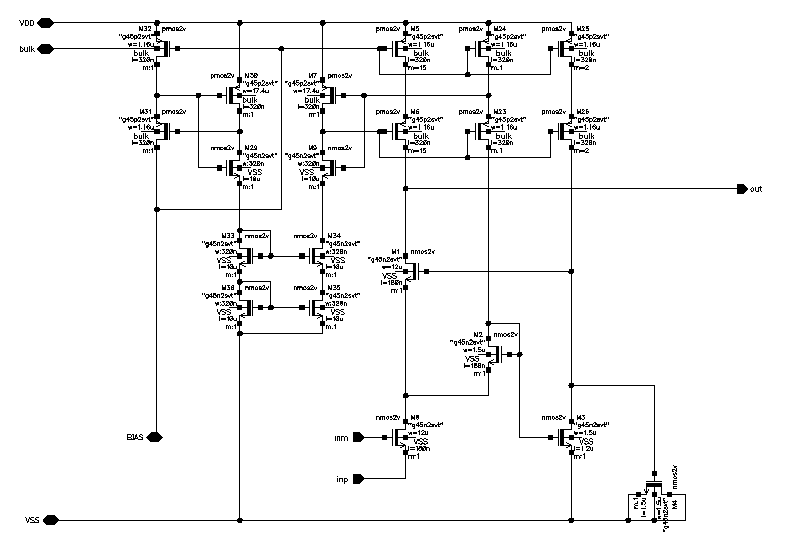
\includegraphics[width=4in]{images/cp_sch_ota.eps} 
    \caption{OTA with wide-swing bias for the charge pump regulator.}\label{fig:ota}
\end{figure}

\subsection{Non-Overlapping Clock}

Since the charge pump circuit relies on keeping the accumulation of charge on the capacitor places as efficient as possible, a non-overlapping generator circuit is used to split a single clock into the two necessary phases and their non-overlapping complements, shown in \cref{fig:clkgen}. The clock used in this design has a \qty{30}{\%} duty cycle to provide some additional efficiency by mostly keeping \(C_{fly}\) in the discharging state. The clock generator uses the a standard configuration with large inverter drivers within the loop to reduce the chance of overlap.

\begin{figure}[ht]
    \centering
    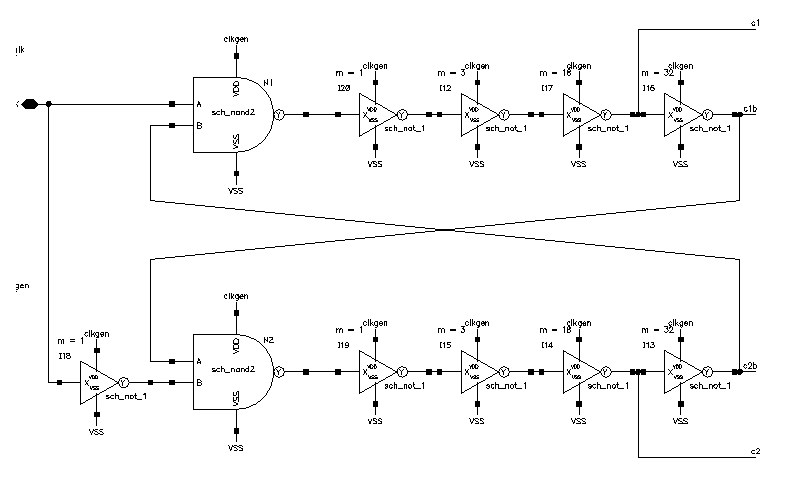
\includegraphics[width=4in]{images/cp_sch_clk.eps} 
    \caption{Non-overlapping clock generator, with multipliers to provide appropriate drive strength for the gigantic switches.}\label{fig:clkgen}
\end{figure}

\subsection{Comparator for Bulk Bias}

Finally, the author has constructed a continuous-time comparator as shown in \cref{fig:comp}. This is used to observe the input and output voltages, and ensure that the PMOS devices of the charge pump and their gate drivers are biased to the highest level to prevent latchup when the input voltage drops and the regulator takes over to keep the output voltage up. The output of the comparator controls t-gates, which appropriately select the bulk bias voltage. To additionally prevent the large devices from being blown up during a shorting event that the comparator does not have time to respond to, resistors are included before the bulk ties. The comparator startup signal is provided by a NOR gate to ensure it is not powered down before \(V_{out}\) discharges below \(V_{bat}\).

\begin{figure}[ht]
    \centering
    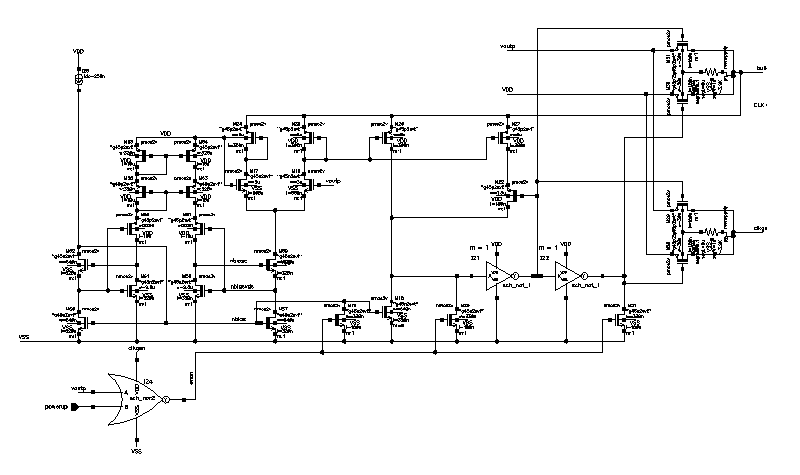
\includegraphics{images/cp_sch_comp.eps}
    \caption{Continuous time comparator for selecting the best PMOS bulk bias voltage.}\label{fig:comp}
\end{figure}

\section{Top-Level Design}

The schematic-level design for this circuit is accomplished with a generously termed ``flattened-hierarchy'' design shown in \cref{fig:sch_full}, which involves dumping everything into a single schematic file. While in no way ideal from an organizational standpoint, this circuit is quite complex and this makes it somewhat easier to navigate all of the connections. The full design is realized using the same normally-open switches from the previous SAR ADC design, with no modification to the t-gate sizes shown in \cref{fig:sch_full}. A single \qty{250}{\nA} reference current is supplied to the current mirror of the comparator, which uses the same mirroring structure as the OTA. This is also mirrored to PMOS devices while being stepped up to \qty{1}{\uA} across the BJT during \(\Phi_1\), \qty{11}{\uA} for \(\Phi_2\), and \qty{10}{\uA} for the charge pump gate drivers. The resistors provided for bulk current limiting are visible on the right side of \cref{fig:sch_full}.

\begin{figure}[ht]
    \centering
    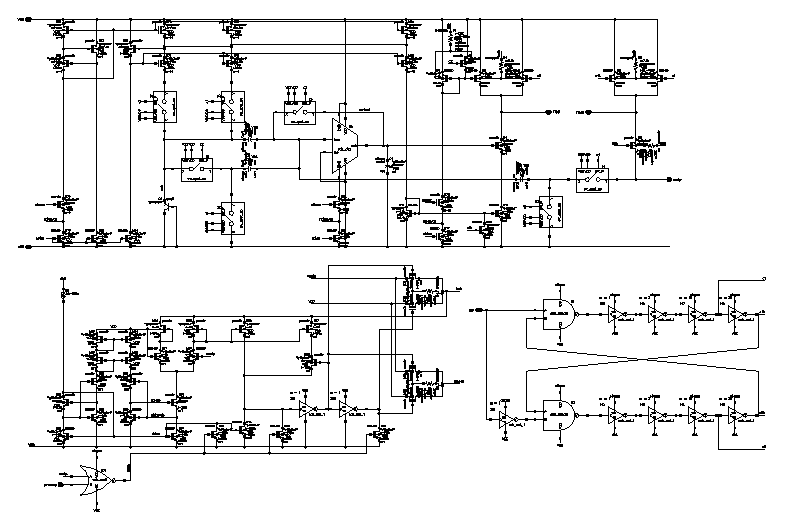
\includegraphics[width=\textwidth]{images/cp_sch_full.eps} 
        \caption{Full regulated charge pump schematic, with accoutrements}\label{fig:sch_full}
\end{figure}

\begin{figure}[ht]
    \centering
    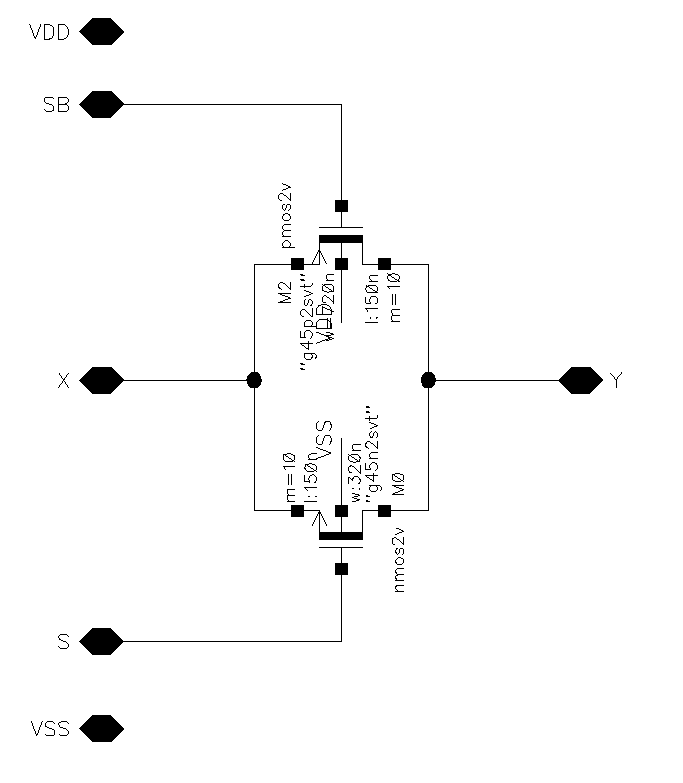
\includegraphics[width=2in]{images/sch_tg.eps} 
    \caption{Transmission gate sizes used for switching in the regulator.}\label{fig:tg_sch}
\end{figure}

\subsection{Device Sizing}

\cref{eq:vref} is used as a starting point to calculate for a \qty{3.3}{\V} nominal output voltage. The ratio of \(C_1\) to \(C_2\) is selected to be 8:1 to target reasonable temperature coefficient correction while enabling 2D common-centroid layout for these important devices. Substitution reveals a subsequent \(\nicefrac{C_2}{C_3}\) ratio of about 2.8, so 28 unit capacitors are chosen for \(C_3\). The unit MIM capacitors for this design are set to \qty{4}{\um} by \qty{4}{\um}, giving a total capacitance of \qty{20.28}{fF} for quick charging. Using \cref{eq:Gm} and setting an arbitrary \(F_{osc}\) of \qty{100}{\mega\Hz}, the size of \(C_4\) can be estimated. Assuming that \(C_{par_{OTA}} \thicksim C_2\), the first term of \cref{eq:Gm} can reduce in terms of \(C_3\) to \(\nicefrac{1}{51.4}\). Using \(\nicefrac{W}{L}\) ratios of \nicefrac{480}{0.18} and assuming \(\mathrm{G_M} \geq 16.5\) is needed for \qty{10}{\%} regulation, it is found through relating \(g_m\) of the OTA to \(C_4\) that \(C_4\) does not need to be large, so 4 times the unit capacitance is selected to start with. The device sizes within the charge pump and comparator are scaled from~\cite{Gregiore2006} down to a minimum length of \qty{180}{\nm} for integer matching. 

\section{Schematic Level Simulations}

This circuit was evaluated at a \qty{40}{\degree\C} nominal corner for schematic simulations. Spectre X simulator is enabled for this design with the AX accuracy preset. The only modifications made to the simulation algorithm are enabling \emph{pivotdc} and \emph{dc\_pivot\_check} to assist the DC solution, and enabling \emph{rebuild\_matrix} to provide more consistency from one run to another. No initial conditions are set on any of the nodes, leaving this to be found by the DC analysis. Transient simulations are performed over a period of \texttt{1000*VAR("Tclk")} while the input is ramped down in voltage to simulate battery discharge while the device is being used. Concrete performance analysis of load and line regulation is somewhat difficult with the parameterized simulation used, so analysis of performance is mostly performed through graphical means.

\subsection{Testbench}

The testbench constructed for the circuit is quite basic, needing only a clock source set up as a pulse with \qty{0.01}{\%} rise and fall times, an enable signal provided by a DC source unless startup behavior is being evaluated, and input power as shown in \cref{fig:tb}. A \qty{1}{\(\upOmega\)} resistor is in series with the ideal voltage source to simulate the typical source impedance of an alkaline battery. The flyback and load filter capacitors are provided by off-chip \qty{100}{\nF} and \qty{1}{\uF} devices, respectively.

\begin{figure}
    \centering
    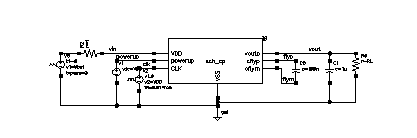
\includegraphics[width=4in]{images/cp_tb.eps}
    \caption{Testbench setup for dropout regulation.}\label{fig:tb}
\end{figure}

\subsection {Results \& Discussion}

Upon the first simulation with ideal current sources, the regulator did appear to perform the regulating, as shown in \cref{fig:firsttry}. As the battery voltage begins to decline, the charge pump does its best to keep the voltage on the output side up close to \qty{3.3}{\V}, until it begins to be loaded down as well. The markers indicate the location of a \qty{10}{\%} drop in output voltage. This simulation was performed with only 100 clock cycles, so the load capacitor does not have time to display it full discharge, but this was great encouragement that the design does work. \cref{fig:firsttry} also shows no kickback onto the input voltage, since this was done before the \qty{1}{\(\upOmega\)} load was added.

\begin{figure}
    \centering
    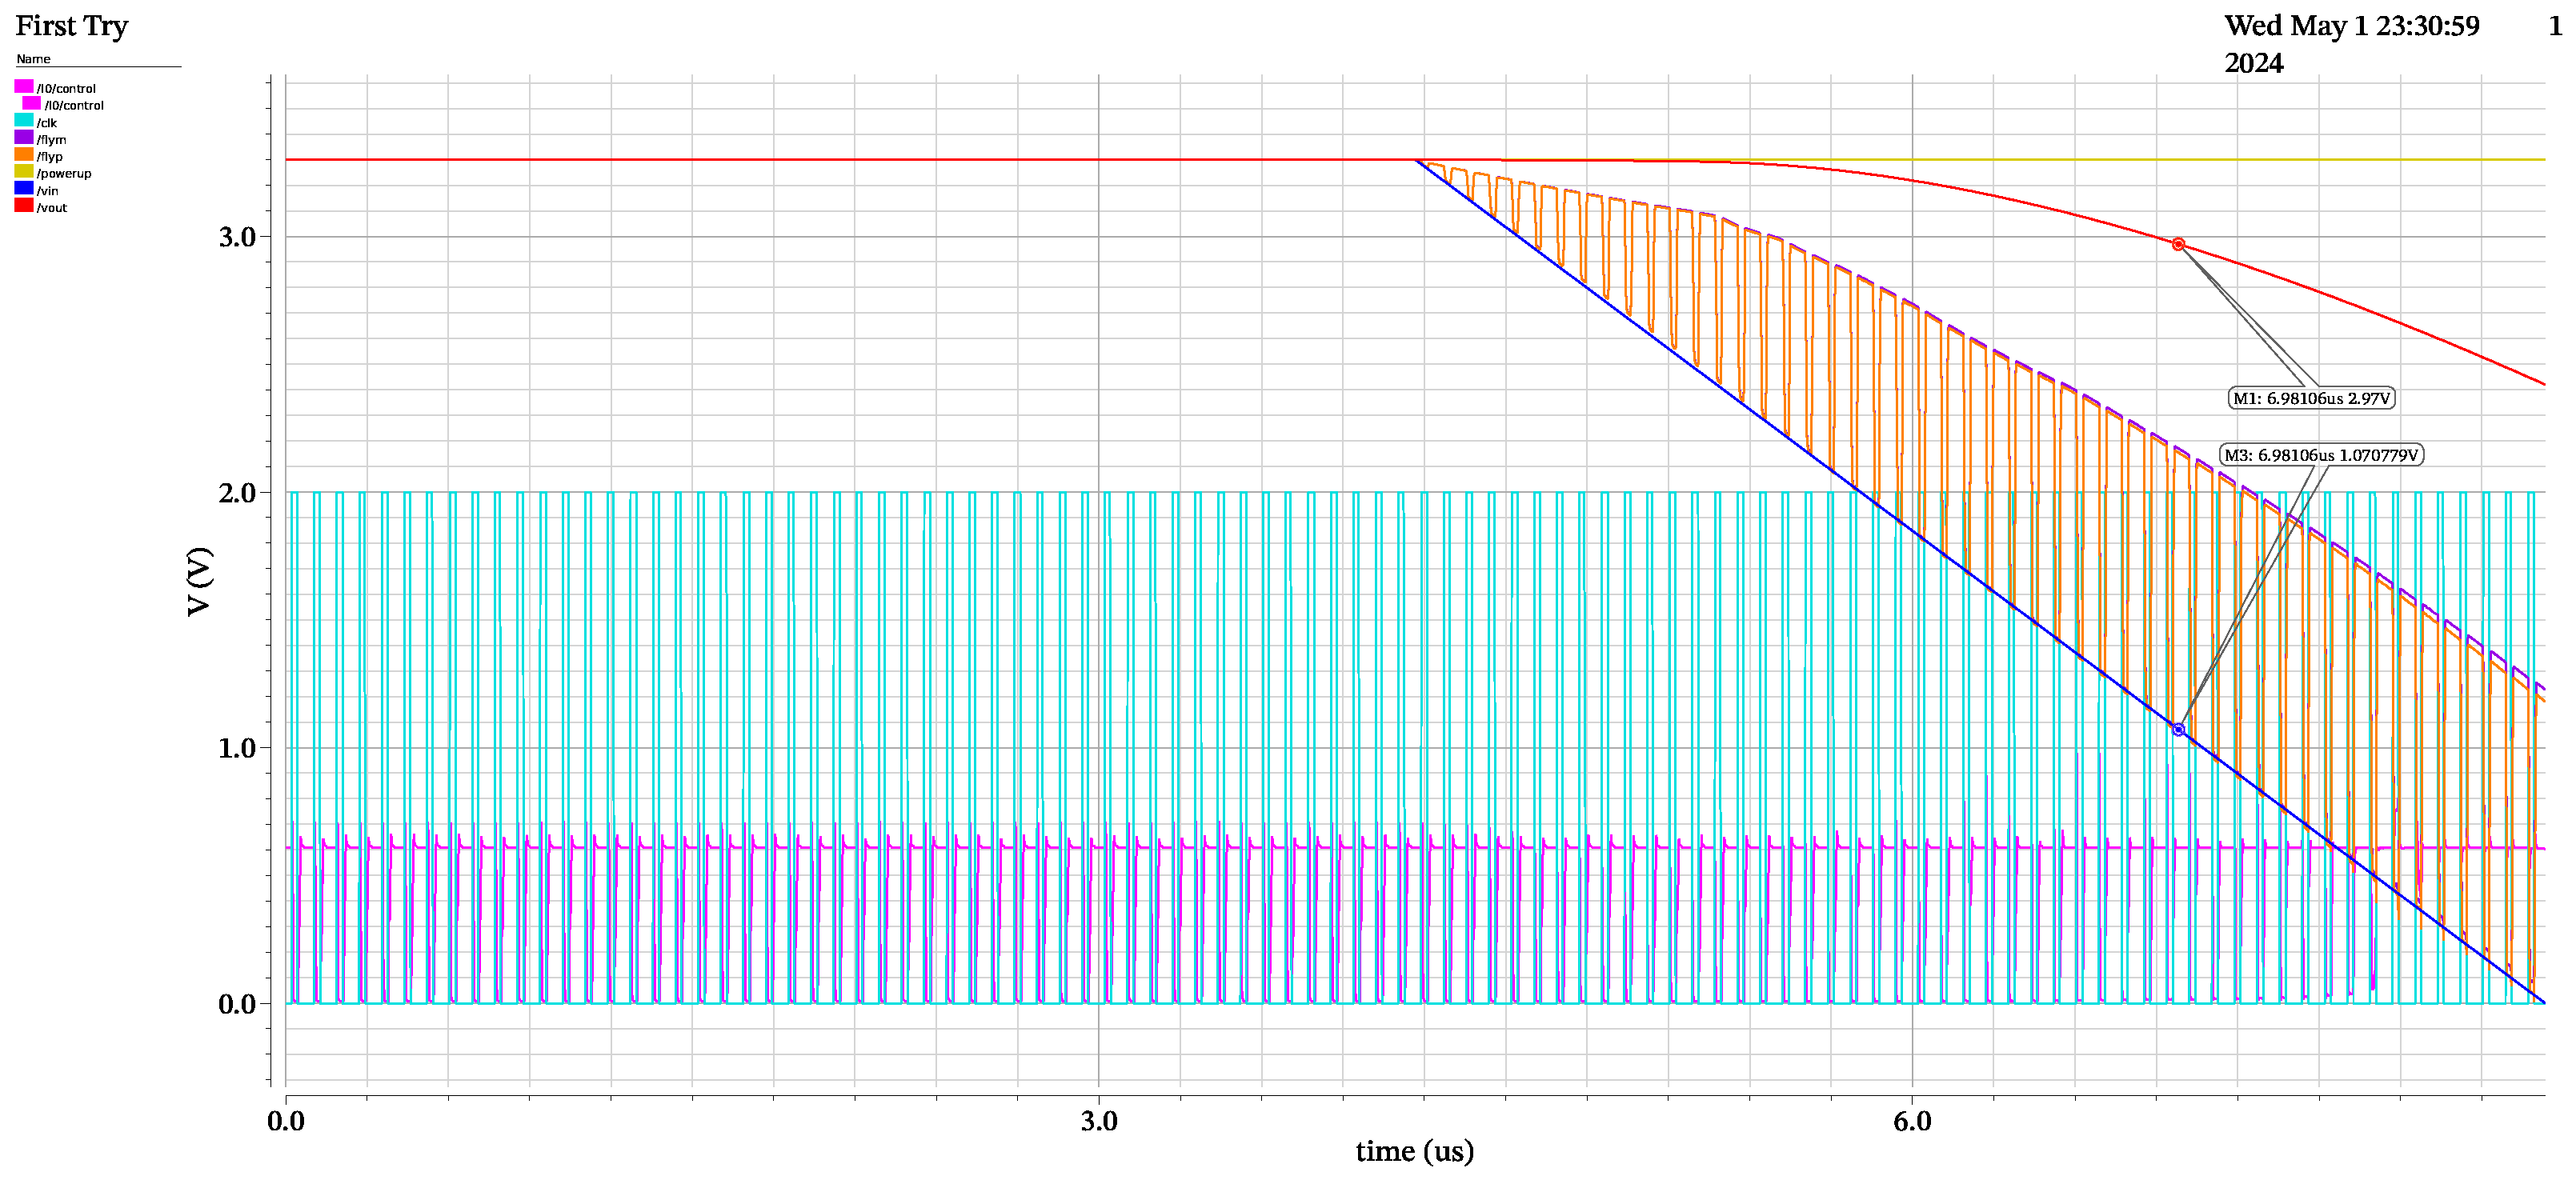
\includegraphics[width=\textwidth]{images/first_try.eps}
    \caption{It works (ideally).}
    \label{fig:firsttry}
\end{figure}

Subsequently, the ideal sources were substituted out for their wide-swing cascoded counterparts. At DC, this configuration performs admirably and ensures very minimal \(V_{DS}\) mismatch in the mirroring devices, so there is minimal change in the bias points for the circuit. Transient simulations also show much the same story, with little to no difference observed in the current/voltage characteristics at the output. From here, 60 simulations are run with 20 different load resistance values from \qty{10}{\(\upOmega\)} to \qty{10}{k\(\upOmega\)} at 0, 40, and \qty{85}{\degree\C}, as shown in \cref{fig:voltage_step}. \cref{fig:current_step} shows the input and output current plots.

\begin{figure}
    \centering
    \includegraphics[width=\columnwidth]{images/step_rl.eps}
    \caption{Input and output voltage plots for different load resistances.}
    \label{fig:voltage_step}
\end{figure}

\begin{figure}
    \centering
    \includegraphics[width=\columnwidth]{images/current_step_rl.eps}
    \caption{Input and output current plots for different load resistances.}
    \label{fig:current_step}
\end{figure}

Overall, performance is better than expected, achieving \qty{10}{\%} dropout at quiescent when driving \qty{48.38}{\mA} into a \qty{61.58}{\(\upOmega\)} load. This is most likely down to some overly cautious estimations made when eyeballing device sizes for the target spec. The output resistance is estimated to be around \qty{10}{\(\upOmega\)} from the plot at which the quiescent output voltage is cut in half. Stability in the frequency domain is ensured with the low output resistance by the high switching frequency and maintaining relatively large capacitors, through the relationship in \cref{eq:stb}.Temperature stability of the circuit is shown to be extremely good, with \qty{0.0112}{\%} variation from 0 to \qty{85}{\degree\C} when driving \(\sim\)\qty{329}{\uA} into \qty{10}{k\(\upOmega\)}, up to \qty{11.65}{\%} variation when driving \(\sim\)\qty{177.3}{\mA} into \qty{10}{\(\upOmega\)}. Since the circuit is not designed to operate at this point, the experienced current stability when operating below \qty{50}{\mA} appears quite sufficient.

Power efficiency calculations proved impossible to get an answer that makes sense from the Cadence calculator, but by observing the plots, about a 2x draw can be seen on the output side as compared to the power supply, which tracks for the behavior of the regulated charge pump. The switching behavior of the bulk bias can also be seen as the input drops below where the output lies, which increases the current draw since the clock power supply is then switched to the more inefficient output side.

While not shown due to data loss associated from what is presumed to be RIT ITS ``technicians'' spilling their coffee into the Cadence server for at least the fourth time this year, or perhaps the computer case overflowing with dust from being improperly cared for, the startup behavior of the circuit was analyzed at the nominal corner. The behavior of the cirucit is as expected; once power is supplied and the startup line pulled high, the filter capacitor on the output begins to charge and takes an appropriate amount of time to reach the full \qty{3.3}{\V}. Reaching full output takes a little bit longer due to the switching behavior, but no unexpected effects are observed.

\section{Layout Floorplan}

To see potential effects of the 3 \(\times\) \qty{1.2}{\mm} transistors on layout area of the circuit, the devices were generated from source within Layout GXL, and the result is shown in \cref{fig:cp_layout}. Surprisingly, even at this scale, the 2 \(\times\) 2 BJT device (the smallest one in the PDK) still dominates in single device size. As auto-generated, the floorplan is \qty{157.64}{\um} square, yielding an area of \qty{24850.37}{\um\squared}. As evidenced in \cref{fig:cp_layout}, there is quite a lot of room for this design to be compacted in layout, or ample space for decap should the designer prefer.

\begin{figure}[tb]
    \centering
    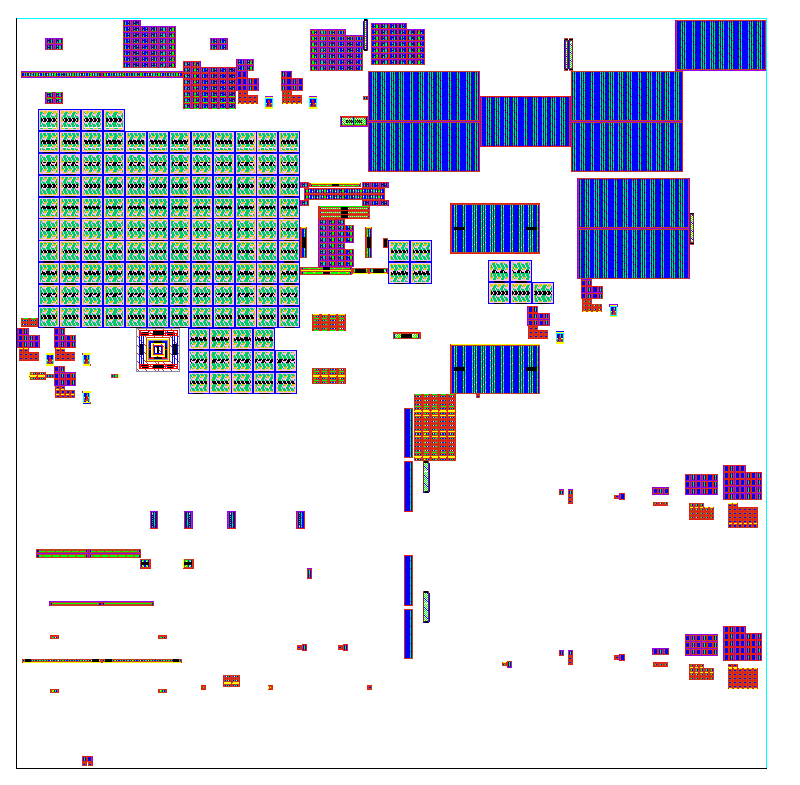
\includegraphics[width=\columnwidth]{images/cp_layout_generated.eps}
    \caption{Device layouts as auto-generated in Layout GXL.}
    \label{fig:cp_layout}
\end{figure}

\section{Conclusion}

For more or less trusting the math laid out by Gregoire on the operation of this circuit, the results obtained by scaling it for the \qty{150}{\nm} PDK and upping the operation speed accordingly appear to be relatively admirable. Benefits of scaling a switched-capacitor design to a small-\(\lambda\) process are nonnegligible and are evidenced in the low output resistance. The extremely solid DC output indicates that the flyback and filter capacitors can be further reduced in size if desired to improve startup time, and possibly be made small enough to integrate on-chip due to running at \qty{100}{\mega\Hz} instead of the \qty{3}{\kHz} in~\cite{Gregiore2006}, which required the bigger capacitors. Approaching this design problem definitely exposed the author to plenty of new areas and ideas in IC design, and there is definitely more work to be done for optimization. Future work on this project would be to incorporate a local clock generator (Johnny or Weston's VCO?) and see how temperature changes cause frequency and output variations, optimize the duty cycle, and fully bootstrap the design so that the \qty{250}{\uA} reference current is provided within this circuit as well, since this would likely be one of the first blocks to receive power within a portable device.

\newpage

\bibliographystyle{bib/IEEEtranDOI}
\bibliography{bib/export.bib}

\newpage

\end{document}